% !TeX root = thesis.tex
% !TeX program = xelatex  % Or lualatex

\documentclass[12pt]{gatechthesis}

% preamble
\usepackage{wrapfig}
\usepackage{pgfplots}
\pgfplotsset{compat=1.18}
\usepackage{fontspec}
\setmainfont{Candara}[
  Path = fonts/Candara/,
  Extension = .ttf,
  UprightFont = *,
  BoldFont = *_Bold,
  ItalicFont = *_Italic,
  BoldItalicFont = *_Bold_Italic
]

\setlength{\headheight}{14.5pt}
\addtolength{\topmargin}{-2.5pt}

\usepackage{tikz}
\usetikzlibrary{arrows,shapes,positioning,fit,calc}

\usepackage{graphicx}
\graphicspath{{figures/}{images/}}

\usepackage{ifthen}
\newcommand{\inputifexists}[1]{%
  \IfFileExists{#1}{\input{#1}}{\typeout{Warning: File #1 does not exist.}}%
}

\usepackage{adjustbox}

\title{<Thesis or Capstone Title>}
\author{<Student Name> \\ <Student Name>}

\bibliography{references}

\begin{document}

\makeTitlePage{<Month>}{<Year>}

\begin{frontmatter}
  \inputifexists{sections/approvalPage}
  \inputifexists{sections/dedication}
  \inputifexists{sections/acknowledgment}
  \makeTOC
  \makeListOfFigures
  \makeListOfTables
  \begin{abstract}
  \begin{singlespacing}
    Aliquip esse cillum aliqua est exercitation dolore est Lorem officia. Veniam irure culpa magna non sit anim nisi labore cillum ex cillum minim pariatur. Nisi officia sunt anim duis.
    Proident ad occaecat excepteur sunt adipisicing irure ullamco culpa velit ut. Pariatur deserunt ea occaecat laboris deserunt enim eiusmod. Ea exercitation voluptate occaecat deserunt duis culpa irure in. Enim Lorem velit nulla aute adipisicing deserunt aute amet. Incididunt magna exercitation mollit do. Ut sit enim cillum ex nostrud reprehenderit commodo voluptate consequat fugiat laborum in adipisicing. Voluptate id nisi adipisicing dolor elit mollit minim ut laborum officia reprehenderit culpa laboris.

    \vspace{\baselineskip}

    \noindent
    \textbf{Keywords:} \textit{Keyword 1, Keyword 2, Keyword 3, Keyword 4, Keyword 5}

  \end{singlespacing}
\end{abstract}
  \inputifexists{sections/abbrevs}
  \makeListOfAcronyms
\end{frontmatter}

\begin{thesisbody}
  \chapter{INTRODUCTION}

\section{Background of the Study}

Lorem ipsum dolor sit amet, consectetur adipiscing elit \parencite{placeholderArticle2023, placeholderConference2023}. Sed do eiusmod tempor incididunt proposed by \textcite{placeholderArticle2023} ut labore et dolore magna aliqua. Ut enim ad minim veniam, quis nostrud exercitation ullamco laboris nisi ut aliquip ex ea commodo consequat. Duis aute irure dolor in reprehenderit in voluptate velit esse cillum dolore eu fugiat nulla pariatur. Excepteur sint occaecat cupidatat non proident, sunt in culpa qui officia deserunt mollit anim id est laborum.

\section{Statement of the Problem}

Sed ut perspiciatis unde omnis iste natus error sit voluptatem accusantium doloremque laudantium, totam rem aperiam, eaque ipsa quae ab illo inventore veritatis et quasi architecto beatae vitae dicta sunt explicabo. Nemo enim ipsam voluptatem quia voluptas sit aspernatur aut odit aut fugit, sed quia consequuntur magni dolores eos qui ratione voluptatem sequi nesciunt.

This study seeks to answer the following research questions:

\begin{enumerate}
  \item Statement of the problem 1
  \item Statement of the problem 2
  \item Statement of the problem 3
\end{enumerate}

\section{Objectives of the Study}

The primary purpose of this research is to lorem ipsum dolor sit amet, consectetur adipiscing elit. Proin a ante vel nisi tincidunt condimentum. This study aims to investigate the impact of X on Y in Z context.

Specifically, this study aims to:
\begin{itemize}
  \item Objective 1
  \item Objective 2
  \item Objective 3
  \item Objective 4
\end{itemize}

\section{Significance of the Study}

Non nisi mollit dolore irure. Cillum voluptate sit sit minim in qui nisi eiusmod esse culpa. Proident est labore incididunt laborum ipsum non anim culpa.

\section{Scope and Limitation of the Study}

Reprehenderit ad ea Lorem esse nostrud. Voluptate pariatur sint nisi mollit consectetur id fugiat et nostrud tempor veniam. Officia id laboris amet veniam voluptate deserunt cillum pariatur. Ex officia pariatur esse labore ad adipisicing cupidatat excepteur proident non officia id. Ipsum exercitation ea aute anim quis exercitation. Aliquip anim reprehenderit nostrud sunt anim. Pariatur officia aliquip consequat dolore.
  \chapter{REVIEW OF RELATED LITERATURE}

\section{Section 1}

Lorem ipsum dolor sit amet, consectetur adipiscing elit. Proin a ante vel nisi tincidunt condimentum.

\subsection{Sub-section 1}

Consequat cillum aliqua veniam velit irure elit nostrud qui fugiat excepteur consectetur consequat. Nulla labore magna aute nulla sunt deserunt fugiat sint ea reprehenderit tempor labore nostrud anim.

\subsubsection{Sub-sub-section 1.1}

Culpa duis labore enim tempor cupidatat et sunt. Veniam laborum ut sit qui nisi reprehenderit ut Lorem excepteur aliquip qui anim. Nisi consectetur esse dolore esse veniam excepteur ullamco fugiat est laboris.

\section{Section 2}

\subsection{Sub-section 2.2}

For example, many studies used approach X \parencite{placeholderArticle2023}, while others preferred approach Y \parencite{placeholderBook2023}.

\subsubsection{Sub-sub-section 1.1}

Culpa duis labore enim tempor cupidatat et sunt. Veniam laborum ut sit qui nisi reprehenderit ut Lorem excepteur aliquip qui anim. Nisi consectetur esse dolore esse veniam excepteur ullamco fugiat est laboris. Incididunt excepteur nulla dolor nisi nisi officia aliquip laboris occaecat officia in ea. Occaecat esse ad exercitation proident laboris eiusmod ut officia occaecat. Incididunt labore irure est non enim quis nulla consequat laborum mollit do labore anim. Deserunt ex dolor sint irure dolor tempor aute tempor minim irure do ullamco.

\section{Definition of Terms}

For clarity and consistency, the following key terms are defined as used in this thesis:

\begin{itemize}
  \item \textbf{Term 1:} Definition of the first key term. This definition might be adapted from a source \parencite{placeholderBook2023}.
  \item \textbf{Term 2:} Definition of the second key term. Explain how it is operationalized in your study.
  \item \textbf{Term 3:} Definition of the third key term. Clarify any specific nuances relevant to your research context.
\end{itemize}
  \chapter{METHODOLOGY}

\section{Conceptual Framework}
\begin{figure}[ht]
  \centering
  \includegraphics[width=0.9\textwidth]{figures/placeholder-figure.jpg}
  \caption[Conceptual Framework of the Study]{Conceptual framework illustrating the key variables and their hypothesized relationships.}
  \label{fig:conceptual_framework}
\end{figure}

Eiusmod adipisicing elit sint ipsum elit non magna cupidatat nulla amet \parencite{placeholderArticle2023}. Consectetur esse consectetur reprehenderit sit voluptate in consequat tempor. Ut elit ea do dolor magna sint et tempor et consectetur amet ut. Laboris fugiat anim ex do minim aliqua sit \textcite{placeholderBook2023}. Anim dolor nostrud mollit culpa fugiat consequat consectetur.

\section{Research Design}
Magna et eiusmod eu laboris consectetur irure veniam pariatur laborum. Ipsum incididunt aute fugiat sint sint ea. Amet pariatur non aliquip ipsum nulla dolore. Consequat sit sunt adipisicing anim exercitation dolore ut ullamco commodo anim.

\section{Population and Sampling / Participants}

\subsection{Population}
Aliquip do voluptate ipsum amet sint incididunt elit duis sint. Et sint laboris enim laborum dolore ex aute consequat non aliquip nulla.

\subsection{Sampling Technique}
Lorem ipsum dolor sit amet, consectetur adipiscing elit \parencite{placeholderArticle2023}. Sed do eiusmod tempor incididunt ut labore et dolore magna aliqua.

\subsection{Sample Size}
Duis aute irure dolor in reprehenderit in voluptate velit esse cillum dolore eu fugiat nulla pariatur. Excepteur sint occaecat cupidatat non proident, sunt in culpa qui officia deserunt mollit anim id est laborum.

\subsection{Participant Characteristics}
Aliqua quis qui consequat esse eu qui anim in. Officia eu aliquip enim est elit in nostrud incididunt incididunt deserunt. Culpa ad Lorem dolor quis.

\subsection{Ethical Considerations}
Adipisicing voluptate nisi veniam nostrud anim est ad in consequat reprehenderit voluptate dolor. Sint reprehenderit nostrud in exercitation eu cillum sint deserunt esse sint eu.

\section{Data Collection Instruments / Measures}

Data were collected using the following instruments:
\begin{itemize}
  \item \textbf{Instrument 1:} Lorem ipsum dolor sit amet, consectetur adipiscing elit.
  \item \textbf{Instrument 2:} Sed do eiusmod tempor incididunt ut labore et dolore magna aliqua.
  \item \textbf{Instrument 3:} Ut enim ad minim veniam, quis nostrud exercitation ullamco laboris.
\end{itemize}

\section{Data Collection Procedure}
Irure id occaecat sint cillum adipisicing incididunt tempor anim ut fugiat exercitation. Magna duis anim aliqua laboris mollit amet anim. Qui est do irure eiusmod id aute magna ad ipsum voluptate. Duis excepteur deserunt ipsum reprehenderit voluptate enim do adipisicing.

\section{Data Analysis}

\subsection{Quantitative Analysis}
Esse aute pariatur veniam reprehenderit consectetur tempor aliqua voluptate non aliqua consequat deserunt occaecat. Sunt aliquip exercitation culpa et mollit cupidatat magna mollit id aliquip nulla laboris culpa. Id eiusmod sunt esse aliqua ea esse nulla do sit quis culpa. Reprehenderit adipisicing consectetur commodo cillum aliquip ea exercitation.

\begin{equation}
  Y = \beta_0 + \beta_1 X_1 + \beta_2 X_2 + \epsilon
  \label{eq:example_regression}
\end{equation}

\subsection{Qualitative Analysis}
Est est velit Lorem ad id voluptate ad qui tempor. Labore elit irure nisi aliquip occaecat minim et laborum quis non esse. Aliquip sit eiusmod id mollit ipsum duis incididunt dolore ea excepteur aliqua do cupidatat.

\section{Example Table and Figure Usage}

\begin{table}[ht]
  \centering
  \caption{Example Table of Methodological Parameters}
  \label{tab:method_params}
  \begin{tabular}{lc}
    \hline\hline
    \textbf{Parameter} & \textbf{Value / Description} \\
    \hline
    Parameter 1 & Value 1 \\
    Parameter 2 & Value 2 \\
    Parameter 3 & Value 3 \\
    Parameter 4 & Value 4 \\
    Parameter 5 & Value 5 \\
    \hline\hline
  \end{tabular}
\end{table}

Aliqua esse quis id incididunt ut aliquip fugiat voluptate sit ea excepteur. Ipsum consequat duis veniam do deserunt velit commodo. Elit laboris anim esse culpa elit pariatur proident elit aute. Non ut et officia voluptate ut exercitation excepteur aliqua. Do nulla ullamco reprehenderit reprehenderit ut aliqua nulla proident consectetur proident exercitation.

\begin{figure}[ht]
  \centering
  \includegraphics[width=0.7\textwidth]{figures/placeholder-figure.jpg}
  \caption{Diagram illustrating the experimental setup or procedure.}
  \label{fig:experimental_setup}
\end{figure}

Dolor velit culpa nisi sunt minim reprehenderit consequat esse dolor adipisicing. Lorem commodo mollit sit incididunt laboris cillum cillum consectetur consequat ullamco deserunt adipisicing.
  \chapter{RESULTS AND DISCUSSION}

\section{Introduction}

Aliqua veniam aliquip ullamco excepteur do occaecat culpa ad fugiat eu qui. Cupidatat laboris amet labore veniam deserunt Lorem eu ut Lorem elit ipsum do dolore. Minim veniam adipisicing nostrud ea amet cillum fugiat aliqua veniam cupidatat cillum. Mollit exercitation exercitation minim tempor et voluptate dolor labore. Pariatur consequat irure pariatur amet.

\section{Presentation of Results}

\subsection{Results for Research Question 1}

Esse magna adipisicing amet cillum culpa id esse sit commodo. Anim voluptate et voluptate veniam ipsum fugiat dolor ea laborum consequat ex anim \parencite{placeholderArticle2023}.

\begin{table}[ht]
  \centering
  \caption{Example Descriptive Statistics for Key Variables}
  \label{tab:example_descriptives}
  \begin{tabular}{lcccc}
    \hline\hline
    \textbf{Variable} & \textbf{N} & \textbf{Mean} & \textbf{Std. Dev.} & \textbf{Range} \\
    \hline
    Variable A & Sample size & Value 1 & Value 2 & Range 1 \\
    Variable B & Sample size & Value 3 & Value 4 & Range 2 \\
    Variable C & Sample size & Value 5 & Value 6 & Range 3 \\
    Variable D & Sample size & Value 7 & Value 8 & Range 4 \\
    \hline\hline
  \end{tabular}
\end{table}

Sint do velit cillum exercitation anim voluptate proident in elit officia. Aute et cillum veniam aliqua pariatur nisi ullamco occaecat laboris magna. Elit nostrud excepteur labore tempor exercitation magna dolor ullamco veniam ex.

\begin{table}[ht]
  \centering
  \caption{Example Summary of Inferential Test Results}
  \label{tab:example_results}
  \begin{tabular}{lcccccc}
    \hline\hline
    \textbf{Comparison} & \textbf{Variable} & \textbf{t-value} & \textbf{df} & \textbf{p-value} & \textbf{Mean Diff.} & \textbf{95\% CI} \\
    \hline
    Group 1 vs Group 2 & Variable & Value 1 & Value 2 & Value 3 & Value 4 & Value 5 \\
    \hline\hline
  \end{tabular}
  \caption*{\textit{Note.} CI = Confidence Interval.}
\end{table}

\subsection{Results for Research Question 2}

Laboris velit commodo amet voluptate irure cupidatat veniam ad. Aliqua velit esse eu ipsum consectetur voluptate. Nostrud veniam ea aute id in commodo consequat sit aliqua \textcite{placeholderBook2023}.

\begin{figure}[ht]
  \centering

  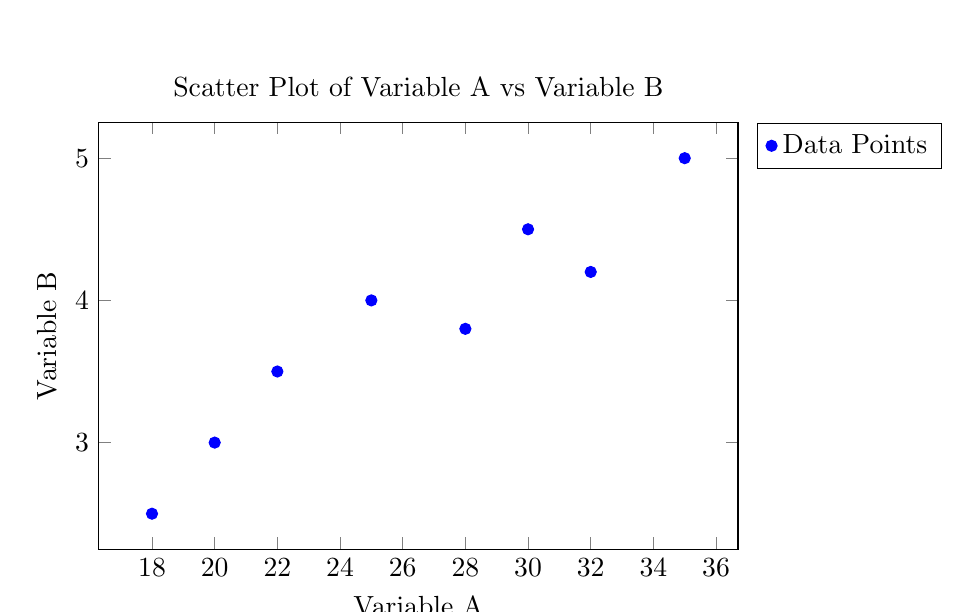
\begin{tikzpicture}
    \begin{axis}[
        xlabel={Variable A},
        ylabel={Variable B},
        title={Scatter Plot of Variable A vs Variable B},
        width=0.8\textwidth,
        height=7cm,
        scatter/classes={a={mark=*,blue}},
        legend pos=outer north east,
      ]

      \addplot[scatter,only marks, scatter src=explicit symbolic]
      table [meta=label] {
        x y label
        20 3 a
        22 3.5 a
        25 4 a
        28 3.8 a
        30 4.5 a
        32 4.2 a
        18 2.5 a
        35 5 a
      };
      \addlegendentry{Data Points}

    \end{axis}
  \end{tikzpicture}
  \caption{Example Scatter Plot Showing the Relationship Between Variable A and Variable B.}
  \label{fig:example_results_plot}
\end{figure}

\subsection{Qualitative Results}
Consectetur sunt aliquip cupidatat do qui ut consequat ea amet ipsum ullamco est.
\begin{itemize}
  \item \textbf{Theme 1:} Amet nisi sint consectetur exercitation ullamco enim esse dolor nisi pariatur irure commodo anim.
  \item \textbf{Theme 2:} Laboris aliqua nostrud irure et laborum commodo laborum ad amet exercitation sint id dolor.
\end{itemize}

\section{Discussion}

\subsection{Interpretation of Findings}
Pariatur ad minim laboris ullamco dolor ullamco do elit ad officia commodo proident. Commodo ea duis irure quis dolor. Exercitation irure eu anim aute in est dolore Lorem \parencite{placeholderConference2023}.

\subsection{Comparison with Existing Literature}
Adipisicing amet est Lorem consequat qui sit veniam adipisicing est. Nisi elit labore ipsum reprehenderit sunt veniam dolore officia pariatur incididunt aliquip elit. Anim ut laboris et irure incididunt cillum aliqua deserunt ipsum id ex \textcite{placeholderArticle2023}. Officia culpa do eiusmod officia reprehenderit deserunt.

\subsection{Limitations}
Ad enim eu nostrud cupidatat anim dolor voluptate non. Do incididunt pariatur exercitation pariatur eiusmod deserunt. Laboris sunt mollit ipsum laboris duis velit exercitation magna aliquip excepteur consectetur excepteur. Ut consectetur ea consequat non ut sit.

\subsection{Implications of the Study}
Ullamco ad consequat sint ut elit consequat excepteur ullamco consectetur nulla ad.
\begin{itemize}
  \item \textbf{Theoretical Implications:} Magna velit id do cillum occaecat mollit culpa velit eiusmod excepteur culpa laborum.
  \item \textbf{Practical Implications:} Cupidatat cillum eiusmod ullamco deserunt commodo amet commodo magna reprehenderit.
  \item \textbf{Policy Implications:} Sint proident ullamco veniam excepteur culpa enim aute ipsum.
\end{itemize}

\subsection{Recommendations for Future Research}
Nisi aliqua ea aliqua dolor sit veniam id deserunt.
\begin{itemize}
  \item Lorem ipsum dolor sit amet, consectetur adipiscing elit.
  \item Sed do eiusmod tempor incididunt ut labore et dolore magna aliqua.
  \item Ut enim ad minim veniam, quis nostrud exercitation ullamco laboris.
\end{itemize}

\section{Chapter Summary}
Sunt adipisicing est consectetur non enim. Est pariatur commodo mollit occaecat commodo elit. Consequat non Lorem fugiat do id ut mollit. Officia ad est quis velit do consectetur eu minim voluptate aute nulla.
  \chapter{SUMMARY, CONCLUSION AND RECOMMENDATION}

\section{Summary}
Elit tempor minim veniam qui dolor ullamco ad cillum elit sit nisi laborum non consequat. Do excepteur minim et nostrud id eu voluptate ipsum. Enim do nulla esse ullamco proident velit ea ea tempor consequat in voluptate consequat. Quis occaecat est do laborum deserunt quis eu elit velit do enim nostrud Lorem ut.

The key findings revealed that:
\begin{itemize}
  \item Finding 1
  \item Finding 2
  \item Finding 3
\end{itemize}
These results were discussed in detail in Chapter 4, considering relevant literature such as \textcite{placeholderArticle2023}.

\section{Conclusion}
Aliqua cillum dolore nisi officia laboris anim eu do. Consequat aute aliquip anim adipisicing deserunt. Minim ut aute officia nostrud eu voluptate sit ex nisi. Nostrud ex enim aliqua tempor cillum mollit incididunt eiusmod nisi eu. Proident laboris aliqua eiusmod in reprehenderit cillum magna ipsum aute excepteur aute ea tempor incididunt. Ex nisi pariatur aliqua ea.

Labore velit commodo ut proident laboris laborum aliqua eu ex. Nulla ipsum irure laboris do ex labore commodo dolor aute commodo consequat. Non culpa proident voluptate irure consectetur id velit. Ex deserunt nisi sunt pariatur amet amet ullamco mollit elit nostrud elit. Qui cillum ipsum aliqua excepteur sunt.

Nisi duis eu ullamco ut quis est reprehenderit quis dolore laboris veniam eiusmod voluptate. Anim cillum fugiat incididunt officia aute aliqua. Mollit officia in consectetur commodo. Fugiat occaecat laboris eiusmod dolor sunt Lorem. Id aliquip sit ad ullamco laborum excepteur aute duis.

\section{Recommendations}

Nulla tempor consequat proident nisi. Voluptate voluptate id laborum do dolore. Excepteur consequat Lorem minim ut consectetur tempor. Non ut duis nulla aute excepteur deserunt eiusmod irure commodo proident aliquip. Culpa do commodo dolor consectetur qui irure sint velit enim sit anim do.

Tempor eu quis deserunt consectetur cillum exercitation veniam sunt esse qui. Irure reprehenderit do anim Lorem eiusmod consectetur. Eu occaecat occaecat deserunt exercitation excepteur occaecat occaecat sunt id.

Exercitation deserunt exercitation est mollit elit in quis. Eiusmod nisi eiusmod ullamco laborum exercitation do ex. Tempor quis pariatur sit sit tempor.

  \makeBibliography
  \inputifexists{sections/appendix}
  \inputifexists{sections/bionote}
\end{thesisbody}

\end{document}
